\section{Microcontroller Clock Drift}
\label{sec:clock_drift}

The Tmote Sky uses a MSP430 microcontroller clocked by an integrated ring oscillator called the \ac{DCO}.
Since the generated clock frequency varies from chip to chip with temperature and operating voltage, the \ac{DCO} can be fine-tuned in software using a modulation functionality.
During booting, TinyOS calibrates the \ac{DCO} using the external low-current \SI{32.756}{\hertz} watch crystal to generate a more accurate \SI{1}{\mega\hertz} clock.
It should be noted, that by default calibration only occurs after a reset, and not periodically during program execution.

We noticed that serial communication stopped working after heating the nodes above $55-$\SI{60}{\celsius}. Below this temperature the problem could be mitigated by resetting the mote to trigger a recalibration of the \ac{DCO}.
Boano~\etal{} reported similar synchronization trouble in their TempLab setup~\cite{Boano2014}.
We therefore looked at the output of the \ac{UART} module with a logic analyzer and measured how the selected baudrate changed over temperature.
The \ac{UART} receiver can tolerate up to $\pm5\%$ relative error, however, with the relative errors of several baudrates reaching well over $-20\%$ as shown in Figure~\ref{fig:baudrate_error}, resynchronization is impossible.

Since the baudrate is generated by scaling the \ac{DCO}, the \emph{relative} baudrate error is equivalent to \emph{relative} \ac{DCO} error over temperature.
We calculated an average temperature clock drift coefficient of \SI{-0.367}{\%\per\celsius}, which is within the typical range according to the datasheet. Similar coefficients were found by Z{\'u}{\~n}iga~\etal~\cite{Zuniga2013}.

\begin{figure}[t]
	\subfigure[Relative error of four baudrates.] {
    	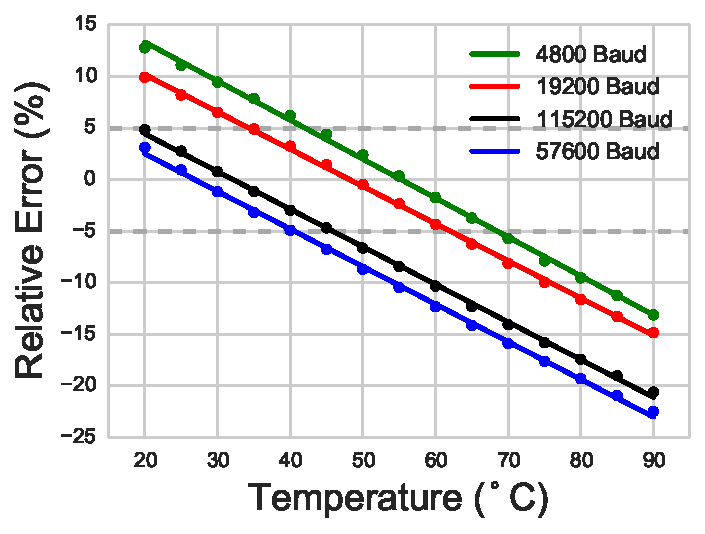
\includegraphics[width=0.475\columnwidth]{figures/baudrate_error}
    	\label{fig:baudrate_error}
    }
    \subfigure[Relative error of \acs{DCO} calibration.] {
	    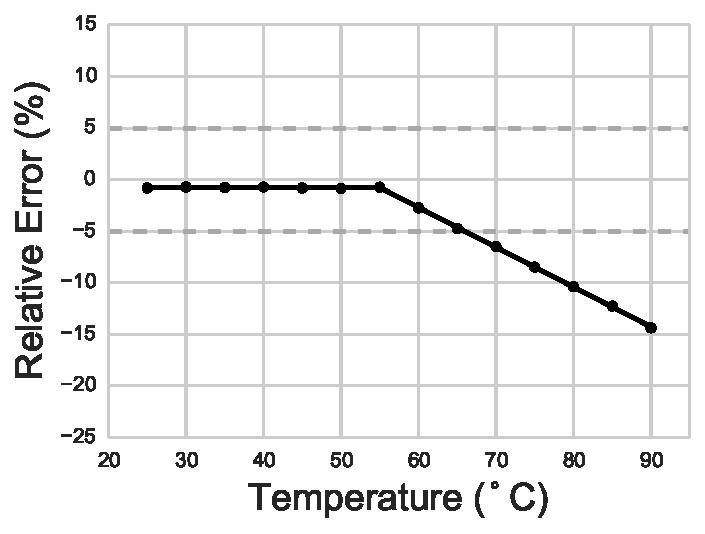
\includegraphics[width=0.475\columnwidth]{figures/reboot_dco_drift}
	    \label{fig:reboot_drift}
	}
	\subfigure[Relative error of corrected baudrate.] {
	    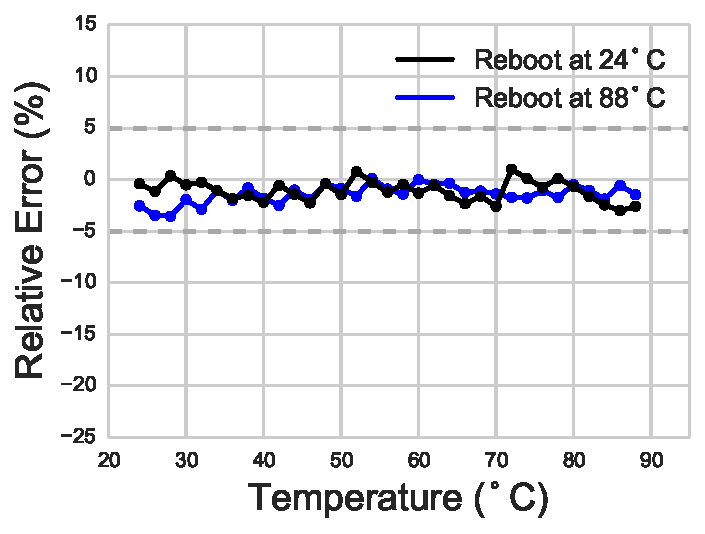
\includegraphics[width=0.475\columnwidth]{figures/baudrate_correction_error}
	    \label{fig:baudrate_look_up_error}
	}
	\subfigure[Values of baudrate correction look-up table.] {
	    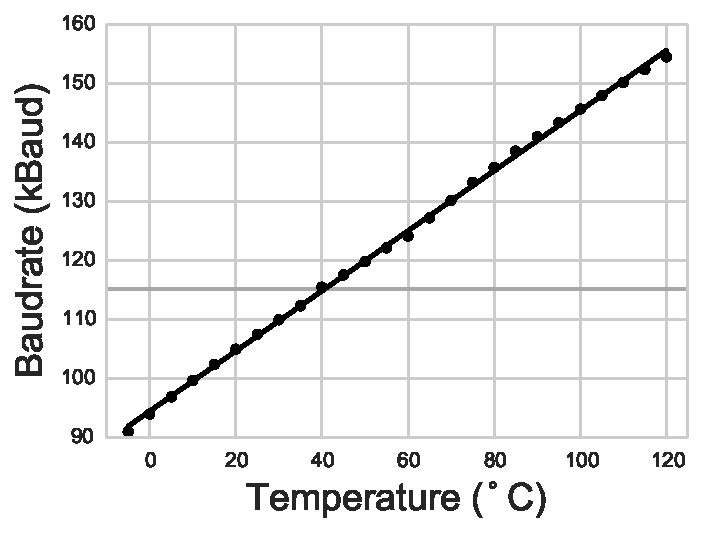
\includegraphics[width=0.475\columnwidth]{figures/baudrate_correction_table}
	    \label{fig:baudrate_look_up}
	}
	\caption{\acs{UART} and \acs{DCO} calibration errors over temperature. The dotted gray line indicates $\pm5\%$ \acs{UART} tolerance.}
\end{figure}

We then measured the relative baudrate error after rebooting over temperature.
As shown in Figure~\ref{fig:reboot_drift}, the TinyOS implementation of the \ac{DCO} calibration only works until \SI{55}{\celsius}, after which it has no corrective effect on CPU frequency, making periodic \ac{DCO} calibration during program execution ineffective.
It is possible that Contiki OS~\cite{contiki-os.org} does not experience these problems as their \ac{DCO} calibration algorithm is different from TinyOS. We did not test this, however.

To not influence the operation of the rest of the microcontroller and since understanding the \ac{DCO} calibration algorithm is not the focus of this thesis, we chose not to correct \ac{DCO} drift directly, but counteract only its effect on baudrate.
To stay within the required tolerance of $\pm5\%$ relative error, we created a fixed lookup-table of ``inverse'' correction baudrates for 115.2kBaud as shown in Figure~\ref{fig:baudrate_look_up}.

Since calculation of prescaler values at runtime is very costly (requiring floating point arithmetic in a recursive algorithm) the look-up table only contains precalculated values, which are then copied into the registers at runtime.
The on-board sensor provides temperature to the \ac{UART} module, which then selects new prescaler values from the look-up table for every \SI{5}{\celsius} temperature difference, which shows up as a sawtooth pattern in Figure~\ref{fig:baudrate_look_up_error} of the resulting relative error of the corrected baudrate.

We used this correction table without change on all of our motes and did not encounter this problem again.
This shows that even with slight differences in clock drift coefficient between different motes, this is approach is enough to solve this issue for our study.

Clock drift is not an issue for the communication between the MSP430 and the CC2420, as it is connected via the \ac{SPI}, which is a synchronous master-slave bus that provides the communication clock for its slaves, requiring no synchronisation on data symbols.
